\documentclass{article}
\usepackage[T1]{fontenc}
\usepackage{lmodern}
\usepackage{graphicx}
\usepackage{amsmath,amssymb}
\usepackage[a4paper,margin=2cm]{geometry}
\usepackage[absolute,overlay]{textpos}
\setlength{\TPHorizModule}{1mm}
\setlength{\TPVertModule}{1mm}
\usepackage[indonesian]{babel}
\usepackage{hyperref}
\setlength{\emergencystretch}{2em}
% unit: Halaman 8

\begin{document}

% === Halaman 8 (llm) ===

\vspace{158.00mm}

\vspace{50mm}
\begin{center}
\textbf{Gambar 2. Algoritma Enkripsi dengan DES}
\end{center}

% deskripsi: Diagram blok proses enkripsi DES yang terdiri dari dua bagian: ringkasan proses di sebelah kiri dan detail iterasi 16 round Feistel di sebelah kanan.
% bbox normalisasi: [0.0370, 0.4300, 0.9270, 0.9620]
\begin{textblock*}{186.90mm}(7.77mm,127.71mm)
\noindent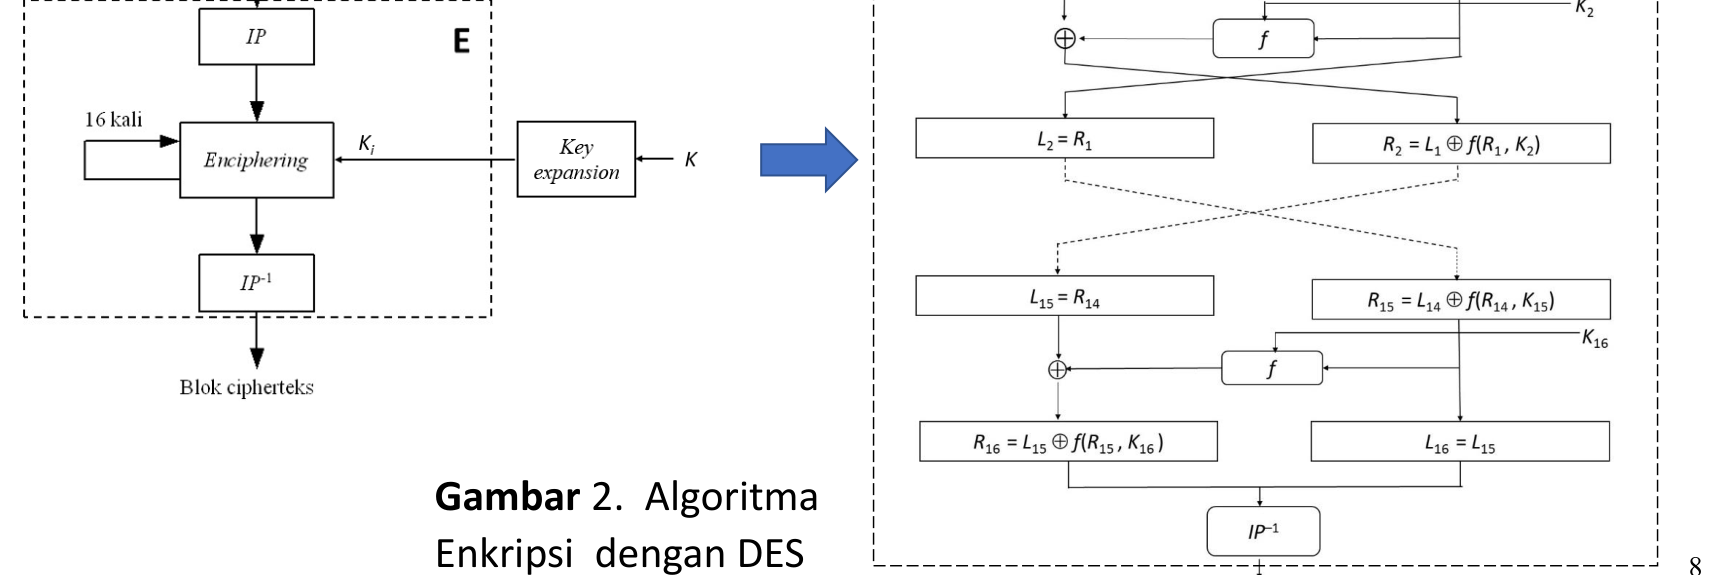
\includegraphics[width=186.90mm,height=158.00mm]{../../images/llm/page_008_img_01.png}%
\end{textblock*}

\end{document}
